\chapter{Group Theory Review}

Symmetry principles play a central role in modern theoretical physics, providing the mathematical foundation for conservation laws and the formulation of fundamental interactions. Group theory offers the natural language to describe these symmetries, both discrete and continuous. In particular, Lie groups and their corresponding algebras form the backbone of relativistic field theories. This chapter reviews the essential concepts of group theory and Lie algebras, culminating in the Lorentz group — the fundamental symmetry group underlying the structure of spacetime in special relativity.

\section*{Definition of a Group}

A \textit{group} is a set \(G\) equipped with a binary operation, denoted by \(\circ\), satisfying four fundamental properties:
\begin{enumerate}
    \item \textbf{Closure:} For any \(a,b \in G\), the product \(a \circ b \in G\).
    \item \textbf{Associativity:} For any \(a,b,c \in G\), one has \((a \circ b) \circ c = a \circ (b \circ c)\).
    \item \textbf{Identity element:} There exists an element \(e \in G\) such that \(e \circ a = a \circ e = a\) for all \(a \in G\).
    \item \textbf{Inverse element:} For each \(a \in G\), there exists \(a^{-1} \in G\) such that \(a \circ a^{-1} = a^{-1} \circ a = e\).
\end{enumerate}

If the operation \(\circ\) is commutative, i.e.\ \(a \circ b = b \circ a\) for all \(a,b \in G\), the group is called \textit{Abelian}.

Typical important groups in physics can be classified as follows:

\begin{itemize}
    \item \textbf{Abelian groups:} groups with commutative operations, often associated with conserved quantities via Noether's theorem.
          \begin{itemize}
              \item \((\mathbb{R}, +)\): additive group of real numbers, e.g., translations in one dimension.
              \item \((\mathbb{C}^\times, \cdot)\): multiplicative group of nonzero complex numbers.
              \item \(\mathrm{U}(1)\): phase rotations, fundamental in electromagnetism and quantum mechanics.
          \end{itemize}

    \item \textbf{Rotation groups:} describe symmetries under rotations in space.
          \begin{itemize}
              \item \(\mathrm{SO}(2)\): rotations in a plane.
              \item \(\mathrm{SO}(3)\): rotations in three-dimensional space, relevant for angular momentum.
              \item \(\mathrm{SU}(2)\times\mathrm{SU}(2)\): cover of \(\mathrm{SO}(3)\), used for spin-$\frac{1}{2}$ particles.
          \end{itemize}

    \item \textbf{Lorentz and Poincaré groups:} spacetime symmetries in relativity.
          \begin{itemize}
              \item \(\mathrm{SO}(1,3)\): Lorentz transformations preserving the Minkowski metric.
              \item \(\mathrm{ISO}(1,3)\) or Poincaré group: Lorentz transformations plus translations, fundamental in field theory.
          \end{itemize}

    \item \textbf{Internal symmetry groups:} act on internal degrees of freedom of fields.
          \begin{itemize}
              \item \(\mathrm{SU(3)}\): color symmetry in quantum chromodynamics.
              \item \(\mathrm{SU(2)} \times \mathrm{U(1)}\): electroweak symmetry in the Standard Model.
          \end{itemize}

    \item \textbf{Discrete groups:} describe symmetries with a finite number of elements.
          \begin{itemize}
              \item Permutation groups \(S_n\), relevant for identical particles and statistics.
              \item Point groups in crystallography and molecular physics.
          \end{itemize}
\end{itemize}

In physics, continuous groups — those depending smoothly on continuous parameters — play a central role, as they describe symmetries of space, time, and dynamical systems. These are known as \textit{Lie groups}.

\section{Lie Groups and Lie Algebras}

A \textbf{Lie group} is a group that is also a smooth differentiable manifold, such that the group operations (multiplication and inversion) are smooth maps.
Lie groups combine the structure of a continuous symmetry with the differentiability properties of manifolds, enabling the use of calculus to study symmetry transformations.

Each Lie group \(G\) is associated with a corresponding \textbf{Lie algebra} \(\mathfrak{g}\), which captures its local (infinitesimal) structure.
Formally, \(\mathfrak{g}\) is defined as \textit{the tangent space to the identity element} \(e \in G\), endowed with a bilinear antisymmetric operation — the \textit{Lie bracket}:
\[
    [\,\cdot\,,\,\cdot\,] : \mathfrak{g} \times \mathfrak{g} \to \mathfrak{g},
\]
which satisfies the Jacobi identity:
\[
    [X,[Y,Z]] + [Y,[Z,X]] + [Z,[X,Y]] = 0, \qquad \forall X,Y,Z \in \mathfrak{g}.
\]

In a neighborhood of the identity, an element of the group is mapped by an exponential map from an element of the Lie algebra:
\[
    g(\epsilon) = e^{i \epsilon^a T_a},
\]
where \(\{T_a\}\) are the \textbf{generators} of the Lie group, and \(\epsilon^a\) are real infinitesimal parameters labeling the transformation.
The commutation relations among generators define the algebraic structure:
\[
    [T_a, T_b] = i f_{ab}{}^{c} \, T_c,
\]
where the real coefficients \(f_{ab}{}^{c}\) are the \textbf{structure constants} of the algebra.

The dimension of a Lie algebra equals the number of independent generators — that is, the number of continuous parameters of the corresponding Lie group.

\textbf{Example:} $SO(2)$ and $\mathfrak{so}(2)$.

\begin{figure}[H]
    \begin{minipage}{0.55\textwidth}
        The group $SO(2)$ represents planar rotations:
        \[
            R(\theta) =
            \begin{pmatrix}
                \cos\theta & -\sin\theta \\
                \sin\theta & \cos\theta
            \end{pmatrix},
            \qquad \theta \in [0,2\pi).
        \]
        Its Lie algebra $\mathfrak{so}(2)$ is the tangent space at the identity, spanned by the generator $J \equiv T_1$:
        \[
            J =
            \begin{pmatrix}
                0 & -1 \\
                1 & 0
            \end{pmatrix},
            \qquad
            R(\theta) = e^{\,\theta J}.
        \]
        The exponential map $\exp: \mathfrak{so}(2) \to SO(2)$ thus identifies each tangent vector $\theta J$ with a rotation of angle $\theta$ on the unit circle.
    \end{minipage}
    \hfill
    \begin{minipage}{0.4\textwidth}
        \centering
        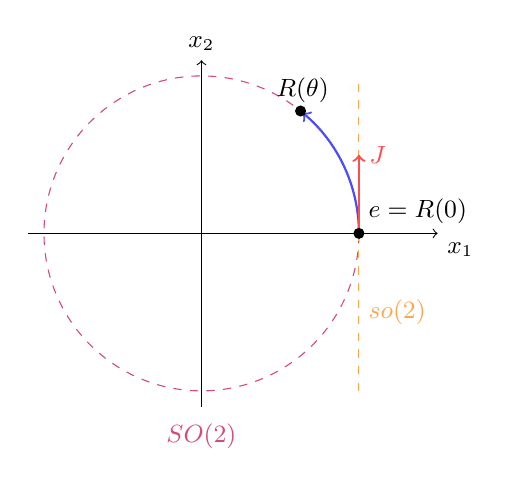
\begin{tikzpicture}[scale=1,every node/.style={font=\small}]
            \draw[->] (-2.2,0) -- (3,0) node[below right] {$x_1$};
            \draw[->] (0,-2.2) -- (0,2.2) node[above] {$x_2$};

            \draw[dashed, purple!70] (0,0) circle (2cm);
            \node[below, purple!70] at (0,-2.3) {$SO(2)$};

            \draw[->, thick, blue!70] (2,0) arc (0:50:2);
            \fill ({2*cos(51)},{2*sin(51)}) circle (2pt);
            \node[above] at ({2*cos(50)},{2*sin(50)}) {$R(\theta)$};

            \draw[dashed,orange!70] (2,-2) -- (2,2);
            \draw[->, red!70, thick] (2,0) -- +(0,1) node[right] {$J$};
            \node[right,orange!70] at (2,-1) {$\mathfrak{so}(2)$};

            \fill (2,0) circle (2pt) node[above right] {$e=R(0)$};
        \end{tikzpicture}
    \end{minipage}
\end{figure}

\textbf{Common Lie groups:}
\begin{itemize}
    \item $\mathbf{O(n)} = \{ R \in \mathbb{R}^{n \times n} \mid R^T R = I \}$: orthogonal group, preserves Euclidean lengths.
    \item $\mathbf{SO(n)} = \{ R \in O(n) \mid \det R = +1 \}$: special orthogonal group, proper rotations in $n$ dimensions.
    \item $\mathbf{U(n)} = \{ U \in \mathbb{C}^{n \times n} \mid U^\dagger U = I \}$: unitary group, preserves complex inner products.
    \item $\mathbf{SU(n)} = \{ U \in U(n) \mid \det U = 1 \}$: special unitary group, important for internal symmetries in particle physics.
          % \item $\mathbf{Sp(2n)} = \{ M \in \mathbb{R}^{2n \times 2n} \mid M^T \Omega M = \Omega \}$: symplectic group, preserves a symplectic form $\Omega$ in classical and quantum mechanics.
\end{itemize}

\subsection{Representations}

A \textbf{representation} of a Lie group or Lie algebra provides a concrete realization of its abstract elements as linear operators acting on a vector space.
Mathematically, a representation of a Lie group \(G\) is a homomorphism, for example
\[
    D : G \to \mathrm{GL}(V),
\]
where \(V\) is the vector space on which our representation is acting and \(\mathrm{GL}(V)\) denotes the group of invertible linear transformations on \(V\).
This means that the group law is preserved:
\[
    D(g_1 g_2) = D(g_1) D(g_2), \qquad \forall g_1,g_2 \in G.
\]
At the infinitesimal level, a representation of the associated Lie algebra \(\mathfrak{g}\) assigns to each generator \(T_a\) a linear operator \(D(T_a)\) such that
\[
    [D(T_a), D(T_b)] = i f_{ab}{}^{c} D(T_c),
\]
mirroring the structure constants \(f_{ab}{}^{c}\) of the algebra.

Representations are fundamental both in mathematics and in physics.
Mathematically, they allow us to study abstract symmetry groups through their action on vector spaces, revealing their structure via matrices or operators.
Physically, they describe how different objects transform under a given symmetry:
scalars correspond to the trivial (one-dimensional) representation,
vectors to the fundamental representation, and spinors or tensors to higher-dimensional or mixed representations.

Of particular importance are the \textbf{irreducible representations}, which cannot be decomposed into smaller invariant subspaces.
These play the role of the "elementary building blocks" of a group—just as elementary particles of definite spin are the basic excitations transforming irreducibly under spacetime symmetries.

Different Lie groups admit representations of various \textbf{dimensions}, depending on how the group acts on the underlying vector space.
For example, the group $SO(2)$ can be represented by $2\times 2$ rotation matrices acting on vectors in the plane, but also by complex phase factors $e^{i n \theta}$ acting on one-dimensional complex spaces, each labeled by an integer $n$.
In general, higher-dimensional representations describe systems that transform with more internal components---such as vectors, tensors, or spinors---while lower-dimensional ones correspond to simpler transformation laws.
The dimension of the representation thus reflects the number of independent degrees of freedom that transform under the symmetry.


\section{The Lorentz Group}

The most fundamental symmetry group in relativistic field theory is the \textbf{Lorentz group}, denoted by \(\mathrm{O}(1,3)\).
It consists of all linear transformations \(\Lambda: \mathbb{R}^{1,3} \to \mathbb{R}^{1,3}\) that leave the Minkowski metric invariant:
\[
    \eta_{\mu\nu} = \mathrm{diag}(1,-1,-1,-1),
\]
i.e.
\[
    \eta_{\mu\nu} \, \Lambda^{\mu}{}_{\rho} \Lambda^{\nu}{}_{\sigma} = \eta_{\rho\sigma}.
\]

These transformations preserve the spacetime interval
\[
    s^2 = \eta_{\mu\nu} x^\mu x^\nu = (x^0)^2 - \vec{x}^{\,2},
\]
or, infinitesimally,
\[
    \mathrm{d}s^2 = \eta_{\mu\nu} \, \mathrm{d}x^\mu \mathrm{d}x^\nu.
\]

Indeed, under a Lorentz transformation \(x^\mu \mapsto x'^\mu = \Lambda^\mu{}_\rho x^\rho\), we have
\[
    \begin{aligned}
        \mathrm{d}s'^2 & = \eta_{\mu\nu} \, \mathrm{d}x'^\mu \mathrm{d}x'^\nu
        = \eta_{\mu\nu} \, \Lambda^\mu{}_\rho \mathrm{d}x^\rho \, \Lambda^\nu{}_\sigma \mathrm{d}x^\sigma                     \\
                       & = \Lambda^\mu{}_\rho \, \eta_{\mu\nu} \, \Lambda^\nu{}_\sigma \, \mathrm{d}x^\rho \mathrm{d}x^\sigma
        = \eta_{\rho\sigma} \, \mathrm{d}x^\rho \mathrm{d}x^\sigma
        = \mathrm{d}s^2,
    \end{aligned}
\]
confirming that Lorentz transformations leave the Minkowski interval invariant.


The determinant of a Lorentz transformation can be either \(+1\) or \(-1\), and \(\Lambda^0{}_0\) can be greater or smaller than \(1\).
The subgroup with \(\det \Lambda = +1\) and \(\Lambda^0{}_0 \ge 1\) is called the \textbf{proper orthochronous Lorentz group}, denoted by \(\mathrm{SO}^+(1,3)\).
It is this connected component that is continuously connected to the identity and relevant for most applications in physics.

\subsection{Infinitesimal Transformations and Generators}

An infinitesimal Lorentz transformation can be written as
\[
    \Lambda^\mu{}_\nu = \delta^\mu{}_\nu + \omega^\mu{}_\nu, \qquad |\omega^\mu{}_\nu| \ll 1,
\]
with the condition
\[
    \eta_{\mu\nu} \Lambda^\mu{}_\rho \Lambda^\nu{}_\sigma = \eta_{\rho\sigma}
    \quad \Rightarrow \quad
    \omega_{\mu\nu} = -\omega_{\nu\mu}.
\]
Hence, \(\omega_{\mu\nu}\) is an antisymmetric tensor containing six independent parameters, corresponding to the six generators of the Lorentz algebra.

We can introduce a set of generators \(M_{\mu\nu}\) (antisymmetric in their indices) such that a general infinitesimal transformation acts on a four-vector \(x^\rho\) as:
\[
    x'^\rho = \left( \delta^\rho{}_\sigma + \frac{i}{2}\,\omega^{\mu\nu} (M_{\mu\nu})^\rho{}_\sigma \right) x^\sigma,
\]
as taylor expansion of
\[
    \Lambda^{\rho}{}_{\sigma} =  e^{\frac{i}{2}\,\omega^{\mu\nu} (M_{\mu\nu})^\rho{}_\sigma},
\]
where the generators of the group are
\[
    (M_{\mu\nu})^\rho_{\ \sigma} = -i \left( \eta_{\mu\sigma} \, \delta^\rho_{\ \nu} - \eta_{\nu\sigma} \, \delta^\rho_{\ \mu} \right),
\]

The commutation relations among the generators define the \textbf{Lorentz algebra} \(\mathfrak{so}(1,3)\):
\[
    [M_{\mu\nu}, M_{\rho\sigma}] = i \left(
    \eta_{\nu\rho} M_{\mu\sigma}
    - \eta_{\mu\rho} M_{\nu\sigma}
    + \eta_{\mu\sigma} M_{\nu\rho}
    - \eta_{\nu\sigma} M_{\mu\rho}
    \right).
\]

\subsection{Generators: Rotations and Boosts}

The six generators can be naturally separated into:
\[
    \begin{aligned}
        J_i & \equiv \frac{1}{2} \epsilon_{ijk} M_{jk} \quad &  & \text{(spatial rotations)}, \\
        K_i & \equiv M_{0i} \quad                            &  & \text{(Lorentz boosts)}.
    \end{aligned}
\]
In terms of these generators, the Lorentz algebra decomposes as:
\[
    [J_i, J_j] = i \epsilon_{ijk} J_k, \qquad
    [J_i, K_j] = i \epsilon_{ijk} K_k, \qquad
    [K_i, K_j] = -i \epsilon_{ijk} J_k.
\]
This structure reveals the non-compact nature of the Lorentz group: unlike spatial rotations, boosts do not form a compact subgroup, as rapidities are unbounded.\footnote{When we later discuss the relation between \(\mathrm{SO}^+(1,3)\) and \(\mathrm{SU}(2) \times \mathrm{SU}(2)\), this distinction will be important: \(\mathrm{SU}(2) \times \mathrm{SU}(2)\) is compact, whereas the proper orthochronous Lorentz group is not.}


For finite transformations, one can write:
\[
    R(\bs{\theta}) = e^{-i \bs{\theta}\cdot \mathbf{J}},
    \qquad
    B(\bs{\beta}) = e^{-i \bs{\beta}\cdot \mathbf{K}},
\]
where \(\bs{\theta} = \left( \theta_1,\,\theta_2,\,\theta_3 \right)\) are the rotation angles and \(\bs{\beta} = \left( \beta_1,\,\beta_2,\,\beta_3\right) \) the boost parameters. We can ultimately reconstruct the expression for \(\omega_{\mu\nu}\):
\[
    \begin{aligned}
        \omega_{ij} & = \epsilon_{ijk}\bs{\theta}^k, \\
        \omega_{0i} & = \bs{\beta}_i.
    \end{aligned}
\]
Together, they parametrize any proper orthochronous Lorentz transformation as a combination of a boost and a rotation:
\[
    \Lambda = B(\bs{\beta}) \, R(\bs{\theta}).
\]

\subsection{Representations}

The Lorentz algebra \(\mathfrak{so}(1,3)\) is locally isomorphic to the direct sum \(\mathfrak{su}(2) \oplus \mathfrak{su}(2)\) (algebra of $SU(2) \times SU(2)$, equivalent up to different hermiticity relations arising because of compactess).
This correspondence allows the classification of all finite-dimensional representations of the Lorentz group in terms of pairs \((j_+, j_-)\) of \(\mathrm{SU}(2)\) spins.

One can then construct the combinations
\[
    \mathbf{A} = \frac{1}{2} (\mathbf{J} + i \mathbf{K}), \qquad
    \mathbf{B} = \frac{1}{2} (\mathbf{J} - i \mathbf{K}),
\]
which satisfy independent \(\mathfrak{su}(2)\) algebras:
\[
    [A_i, A_j] = i \epsilon_{ijk} A_k, \quad
    [B_i, B_j] = i \epsilon_{ijk} B_k, \quad
    [A_i, B_j] = 0.
\]

This shows explicitly the algebra decompiìosition into a direct sum of two commuting algebras.
A concrete realization of the Lorentz algebra generators can be constructed using \textbf{spinor spaces}.
Consider spin-$\tfrac{1}{2}$ representations, and let \(\sigma_i\) denote the Pauli matrices.
Define the combinations
\[
    \mathbf{A} = \frac{1}{2} \boldsymbol{\sigma} \otimes \mathbf{1}, \qquad
    \mathbf{B} = \frac{1}{2} \mathbf{1} \otimes \boldsymbol{\sigma},
\]
which act on the four-dimensional space \(\mathbb{C}^2 \otimes \mathbb{C}^2\).

In this language, the \textbf{left-handed} (LH) \textbf{spinors} transform under the \((\tfrac{1}{2},0)\) representation, corresponding to the action of \(\mathbf{A}\) on the first factor, while the \textbf{right-handed} (RH) \textbf{spinors} transform under the \((0,\tfrac{1}{2})\) representation, corresponding to the action of \(\mathbf{B}\) on the second factor.

The Dirac spinor arises as the direct sum \(\psi = \psi_L \oplus \psi_R \in \mathbb{C}^2 \oplus \mathbb{C}^2\), and higher-dimensional representations of the Lorentz group can be constructed by taking tensor products of these spinor spaces, yielding \((j_+, j_-)\) representations with arbitrary spins.

\paragraph{Trivial representation.}
In addition to the nontrivial representations, every Lie group admits a trivial representation, denoted by $(0,0)$ in the $\mathrm{SU}(2)\times\mathrm{SU}(2)$ classification. In this representation, the group acts identically on the vector space: for any group element $g \in G$ and any vector $v$ in the representation space,
\[
    g \cdot v = v.
\]
The trivial representation is one-dimensional and corresponds to \textit{scalars} under the symmetry: objects that remain invariant under all group transformations, such as the Higgs field under Lorentz transformations.

Although the underlying representation space $\mathbb{C}^2 \otimes \mathbb{C}^2$ is the same, different choices of the $(j_+,j_-)$ representation allow us to classify distinct particles and fields according to their transformation properties under the Lorentz group, as shown in the following table.

\begin{table}[H]
    \centering
    \begin{tabular}{clc}
        \toprule
        Representation $(j_+,j_-)$               & Field / Particle type   & Total spin $s$ \\
        \midrule
        $(0,0)$                                  & Scalar                  & $0$            \\
        $\left(\tfrac{1}{2},0\right)$            & LH Weyl spinor          & $\tfrac{1}{2}$ \\
        $\left(0,\tfrac{1}{2}\right)$            & RH Weyl spinor          & $\tfrac{1}{2}$ \\
        $\left(\tfrac{1}{2},0\right)\oplus\left(0,\tfrac{1}{2}\right)$
                                                 & Dirac spinor            & $\tfrac{1}{2}$ \\
        $\left(\tfrac{1}{2},\tfrac{1}{2}\right)$ & Vector                  & $1$            \\
        $\left(1,\tfrac{1}{2}\right)\oplus\left(\tfrac{1}{2},1\right)$
                                                 & Rarita--Schwinger field & $\tfrac{3}{2}$ \\
        $(1,1)$                                  & Graviton                & $2$            \\
        \bottomrule
    \end{tabular}
\end{table}
The representations listed above correspond to the basic field types used in relativistic quantum field theory. Scalars describe spinless particles such as the Higgs boson. Weyl spinors transform under chiral representations of the Lorentz group, and their direct sum forms the Dirac spinor, which accounts for massive spin-$\tfrac{1}{2}$ fermions like the electron. The vector representation corresponds to spin-1 gauge bosons, such as the photon or gluons. The Rarita--Schwinger field describes spin-$\tfrac{3}{2}$ particles, notably the gravitino in supersymmetric theories, while the symmetric rank-2 tensor representation corresponds to the graviton, a hypothetical spin-2 quantum of the gravitational field.

This representation theory is the foundation for classifying relativistic fields and particles by their transformation properties under the Lorentz group.
